\documentclass{beamer}
\usepackage[utf8]{inputenc}
\usepackage{graphics}
\usepackage{subfig}
\usepackage{wrapfig}
\usepackage{amsmath, amssymb, amsthm}
\usepackage{xcolor}
\usepackage{mathtools}

\usetheme{Warsaw}
\setbeamercovered{transparent} % transparent after pause
\setbeamertemplate{caption}[numbered] % numbered figures
\setbeamertemplate{navigation symbols}{} %remove navigation symbols
\addtobeamertemplate{navigation symbols}{}{ % add page numbers instead
    \usebeamerfont{footline}%
    \usebeamercolor[fg]{footline}%
    \hspace{1em}%
    \insertframenumber/\inserttotalframenumber
}
\AtBeginSection{\frame{\sectionpage}} % add automatic section title frames

\usefonttheme[onlymath]{serif} % set math font
\definecolor{mathcolor}{RGB}{0,0,255} % define math color
\setbeamercolor{math text}{fg=mathcolor} % set in-text math color
\setbeamercolor{math text displayed}{fg=mathcolor} % set display math color
\addtobeamertemplate{frametitle}{\donotcoloroutermaths} % cancel math coloring in frame titles

% General shortcuts
\newcommand{\Ee}{\mathbb{E}}
\newcommand{\Pp}{\mathbb{P}}
\newcommand{\Vv}{\mathbb{V}}
\newcommand{\Rr}{\mathbf{R}}
\newcommand{\one}{\mathbf{1}}
\newcommand{\intd}{\mathrm{d}}

% Problem-specific notation
\newcommand{\X}{\mathbf{X}}
\newcommand{\probaspace}{\mathcal{P}}
\newcommand{\F}{\mathcal{F}}
\newcommand{\Ll}{\mathbb{L}}
\newcommand{\identity}{\mathrm{i}}
\newcommand{\allF}{\mathfrak{F}}
\newcommand{\transportdistance}{\mathsf{d}_{\mathsf{transport}}}
\newcommand{\multistagedistance}{\mathsf{d}_{\mathsf{multistage}}}
\newcommand{\nesteddistance}{\mathsf{d}_{\mathsf{nested}}}
\newcommand{\leaves}{\mathrm{leaves}}

\title[The Fast Bilateral Solver]{\textit{The Fast Bilateral Solver}
- Barron \& Poole}
\author{Guillaume Dalle}
\institute{MVA - Imagerie numérique}
\date{16/01/2019}

\begin{document}

\begin{frame}
\titlepage
\end{frame}

\section{Model and algorithm}

\subsection{Mathematical formulation}

\begin{frame}{Edge-aware smoothing}

We want to create an image $\textbf{x}$ that:
\begin{itemize}
    \item Stays close to a target $\textbf{t}$ in terms of its channel values
    \item Respects the structure of a reference $\textbf{p}$
\end{itemize}

\pause
Optimization problem:
$$\min_{x \in \textbf{R}^N} \frac{\lambda}{2} \sum_{1 \leq i, j \leq N}{\hat{W}_{i, j} (x_i - x_j)^2} + \sum_{1 \leq i \leq N}{c_i (x_i - t_i)^2}$$
where $W_{ij}$ measures the similarity (in terms of color and location) between two pixels $i,j$ of $\textbf{p}$.

\pause
BUT $\textbf{x}$ is too large to solve this problem.
\end{frame}

\begin{frame}{Splat-blur-slice}
\begin{figure}
\centering
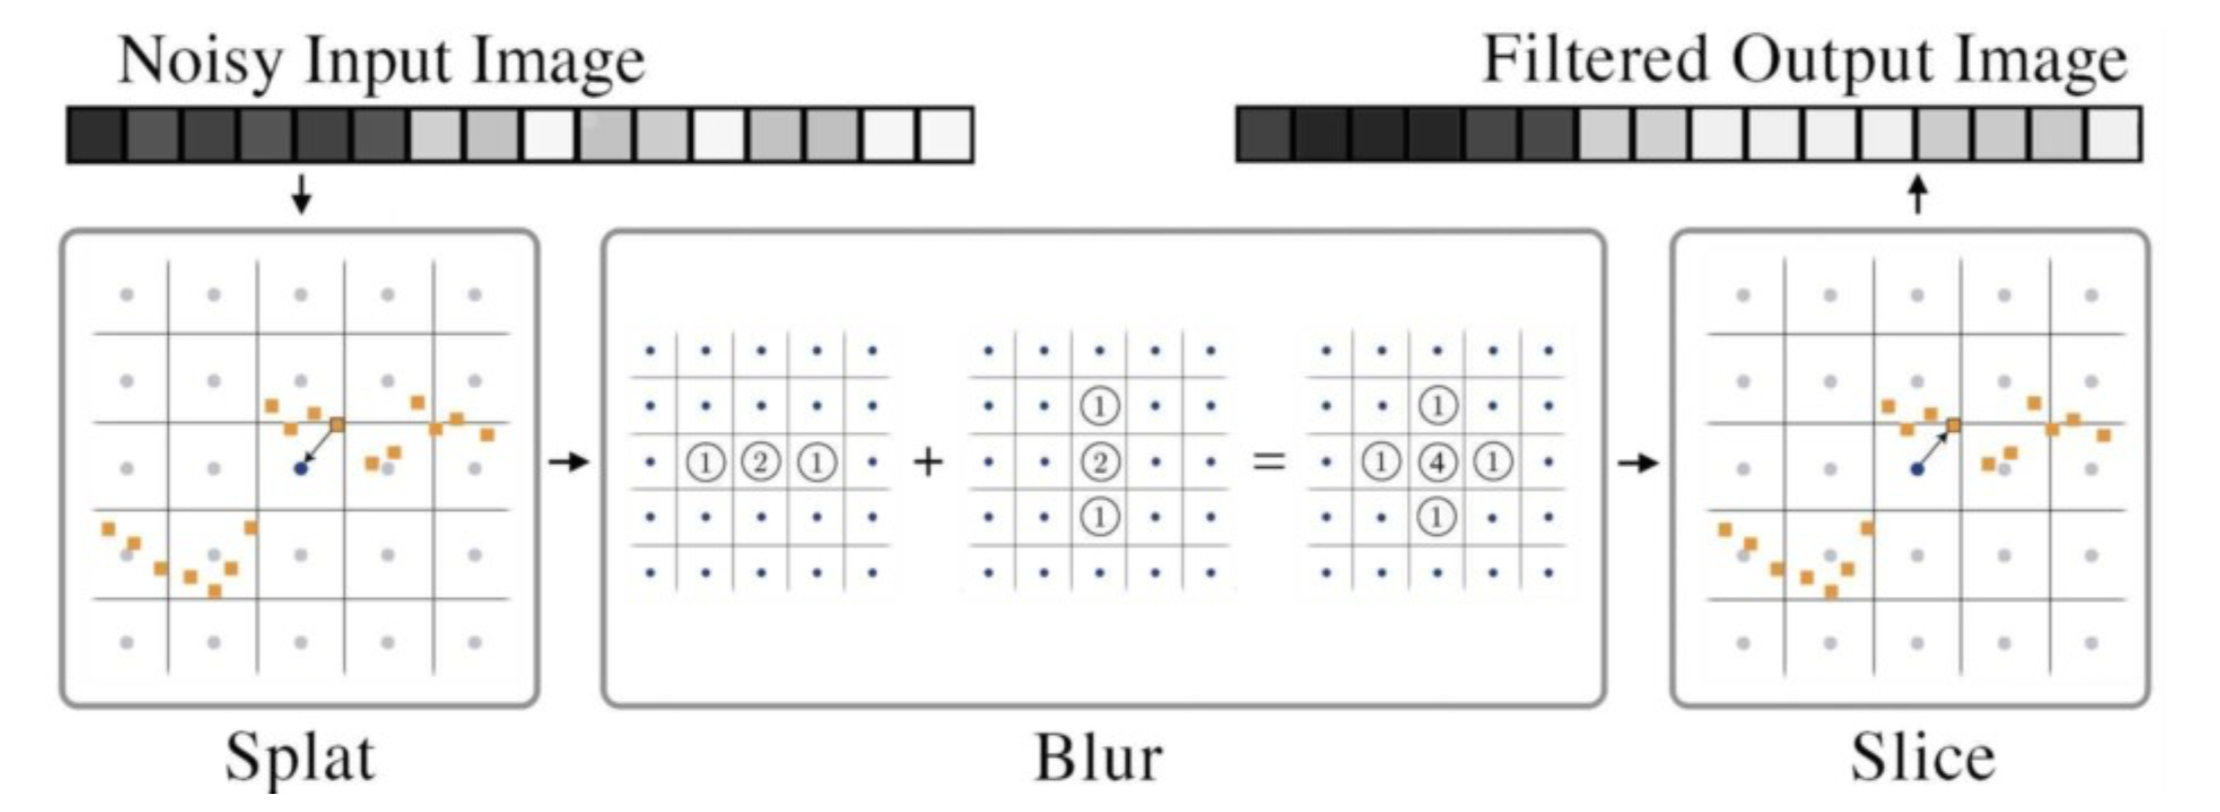
\includegraphics[width=\linewidth]{pictures/SBS.png}
\caption{Illustration of the splat-blur-slice procedure on a 1D image}
\end{figure}

\pause
This can be seen as a factorization $W \simeq S^T B S$.

We can solve the optimization problem in bilateral space, using variable $\textbf{y} = S \textbf{x}$: huge dimension reduction!
\end{frame}

\subsection{Implementation details}

\section{Some applications}

\subsection{Cartooning and sharpening}

\begin{frame}{Cartooning and sharpening}

\only<1>{
\begin{figure}
    \centering
    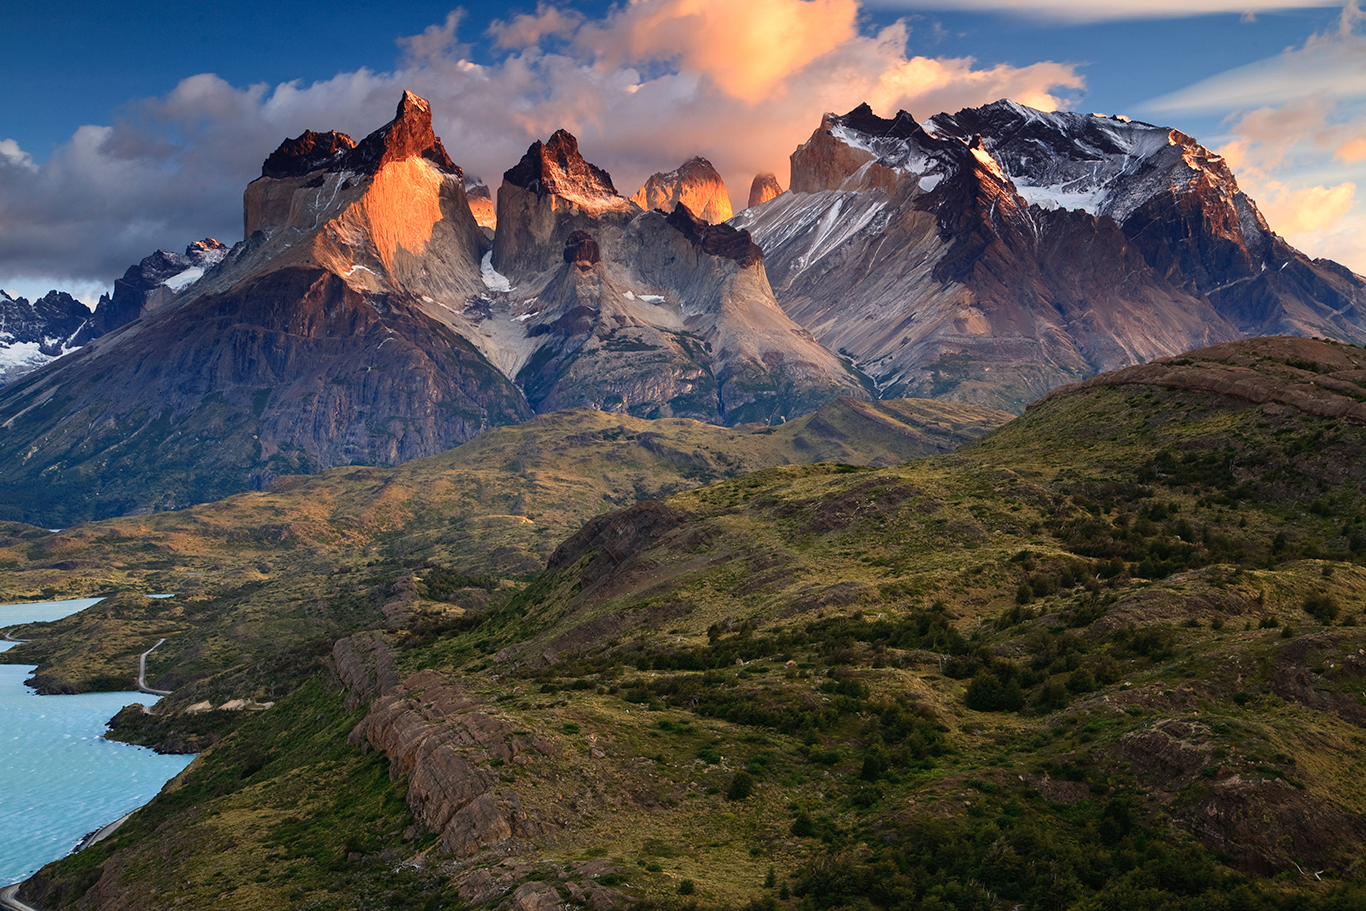
\includegraphics[width=0.45\linewidth]{..code/results/smoothing_landscape_ref.png}
    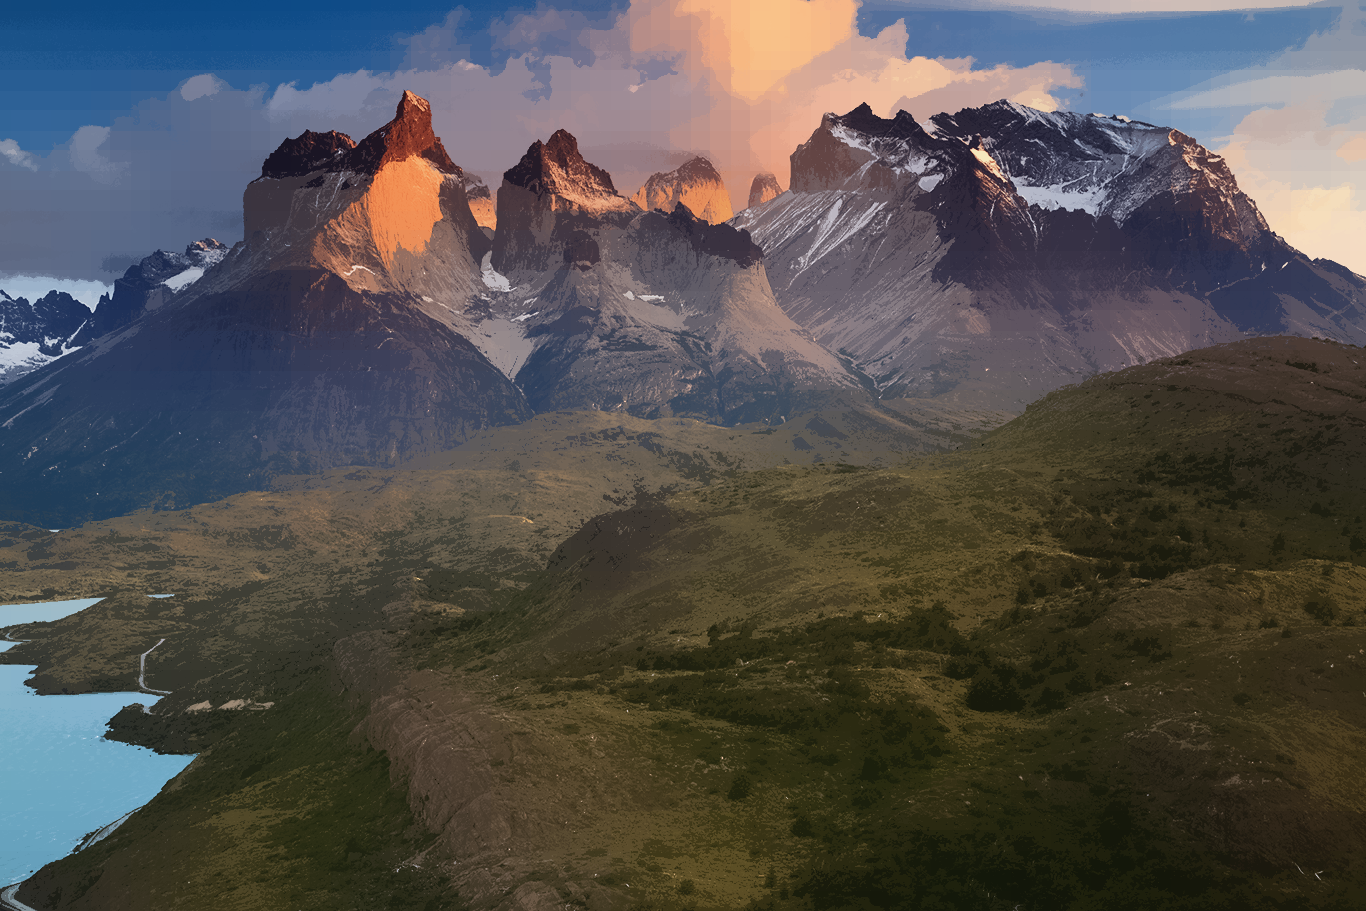
\includegraphics[width=0.45\linewidth]{..code/results/smoothing_landscape_new.png}
    \caption{Result of cartooning}
    {\it Left: original picture. Right: smoothed version.}
\end{figure}
}

\only<2>{
\begin{figure}
    \centering
    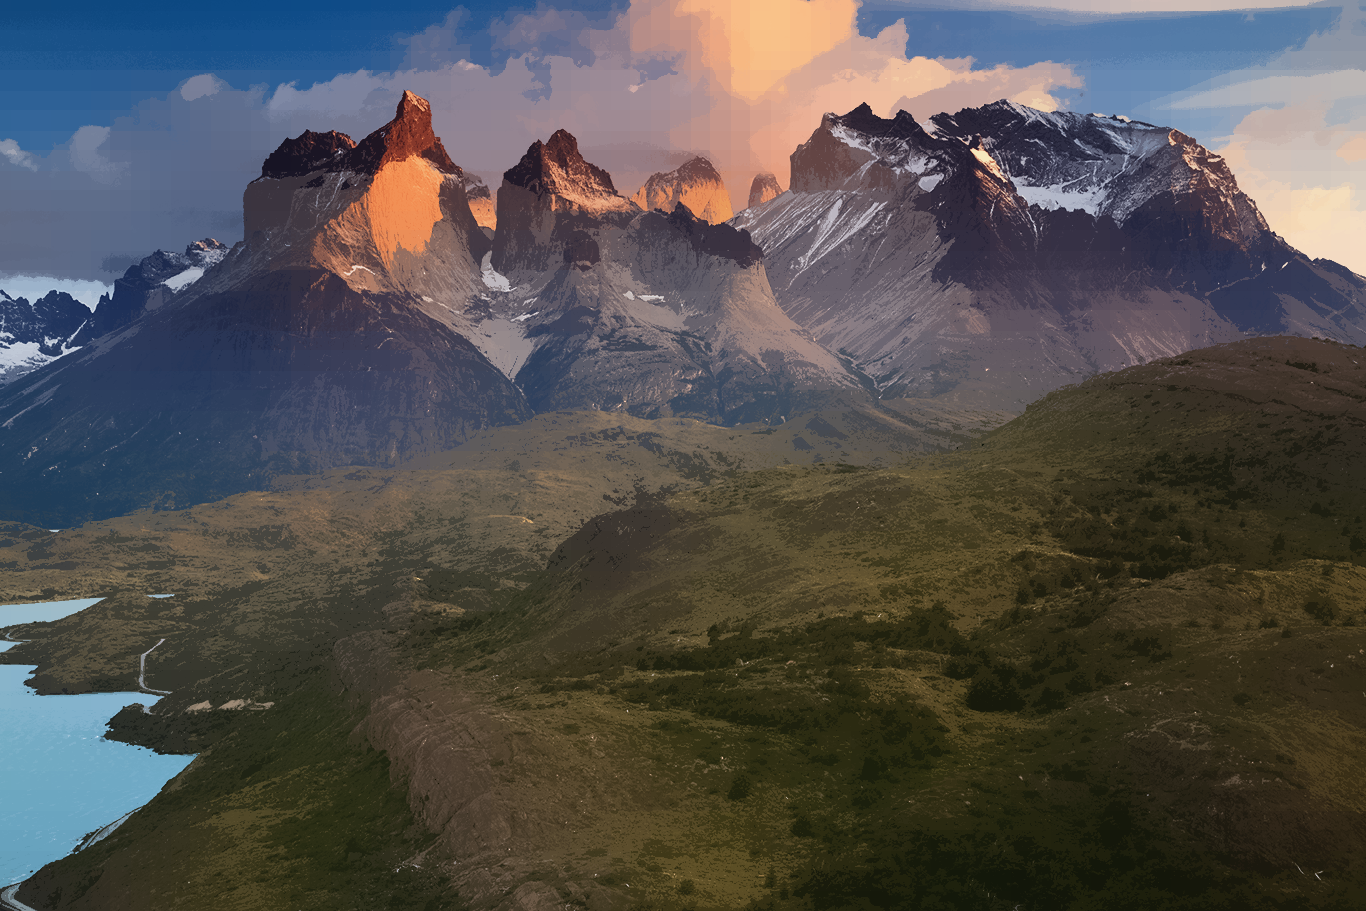
\includegraphics[width=0.45\linewidth]{..code/results/smoothing_landscape_new.png}
    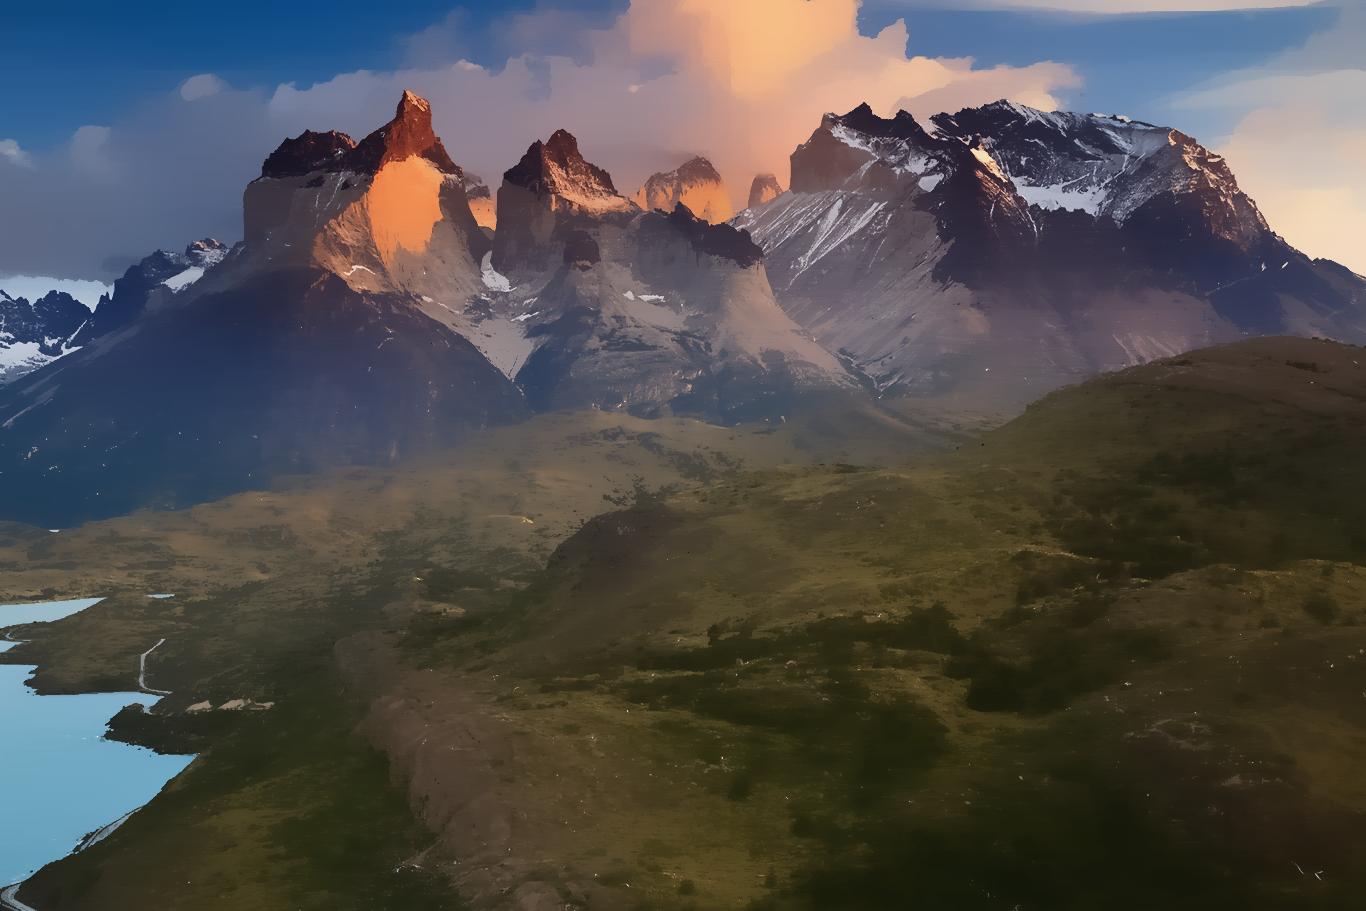
\includegraphics[width=0.45\linewidth]{..code/results/smoothing_landscape_DT_new.png}
    \caption{Result of domain transform post-processing}
    {\it Left: smoothed with FBS. Right: smoothed with FBS + DT.}
\end{figure}
}

\only<3>{
\begin{figure}
    \centering
    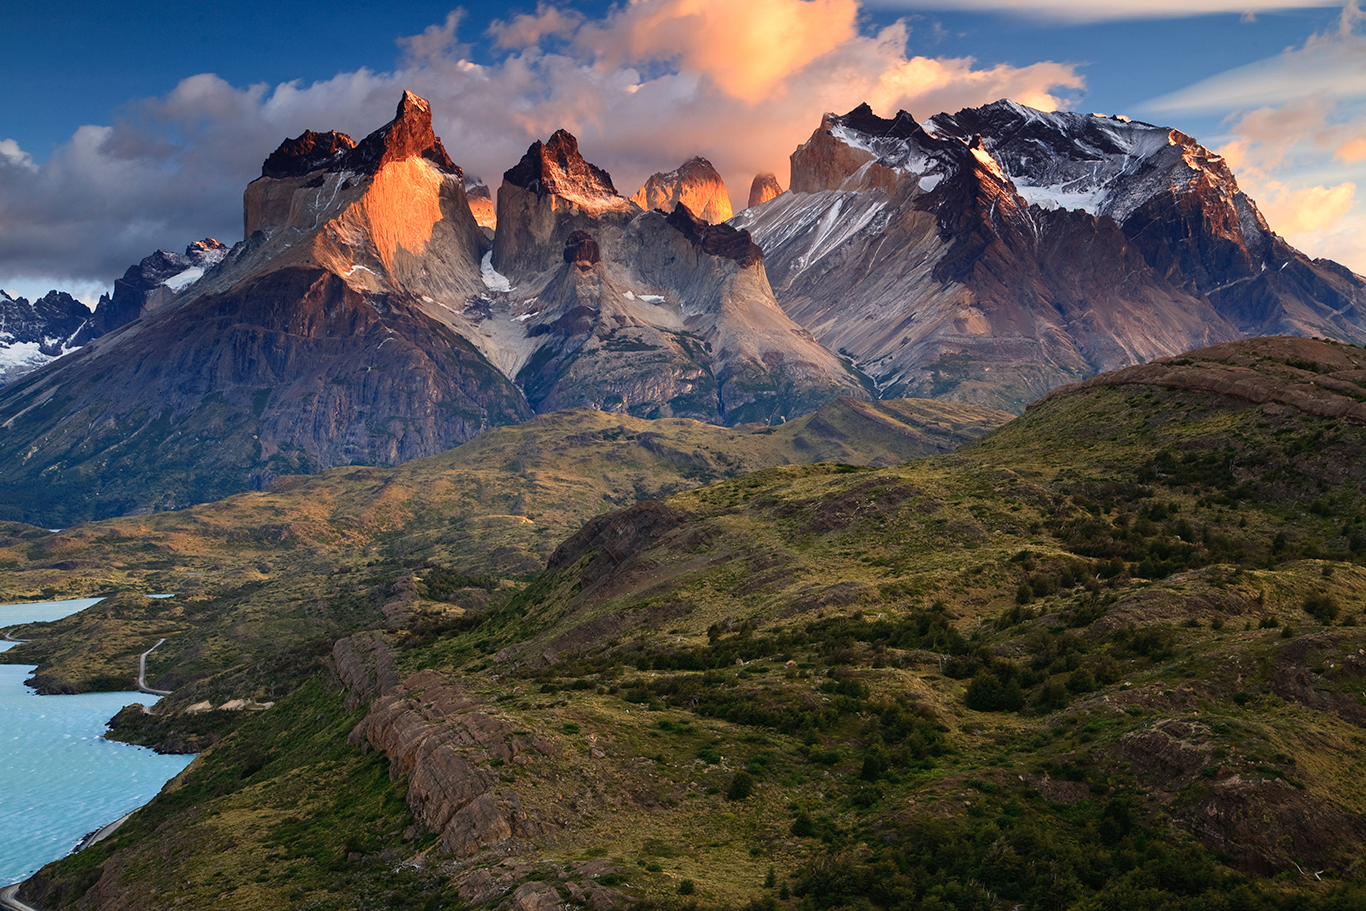
\includegraphics[width=0.45\linewidth]{..code/results/smoothing_landscape_ref.png}
    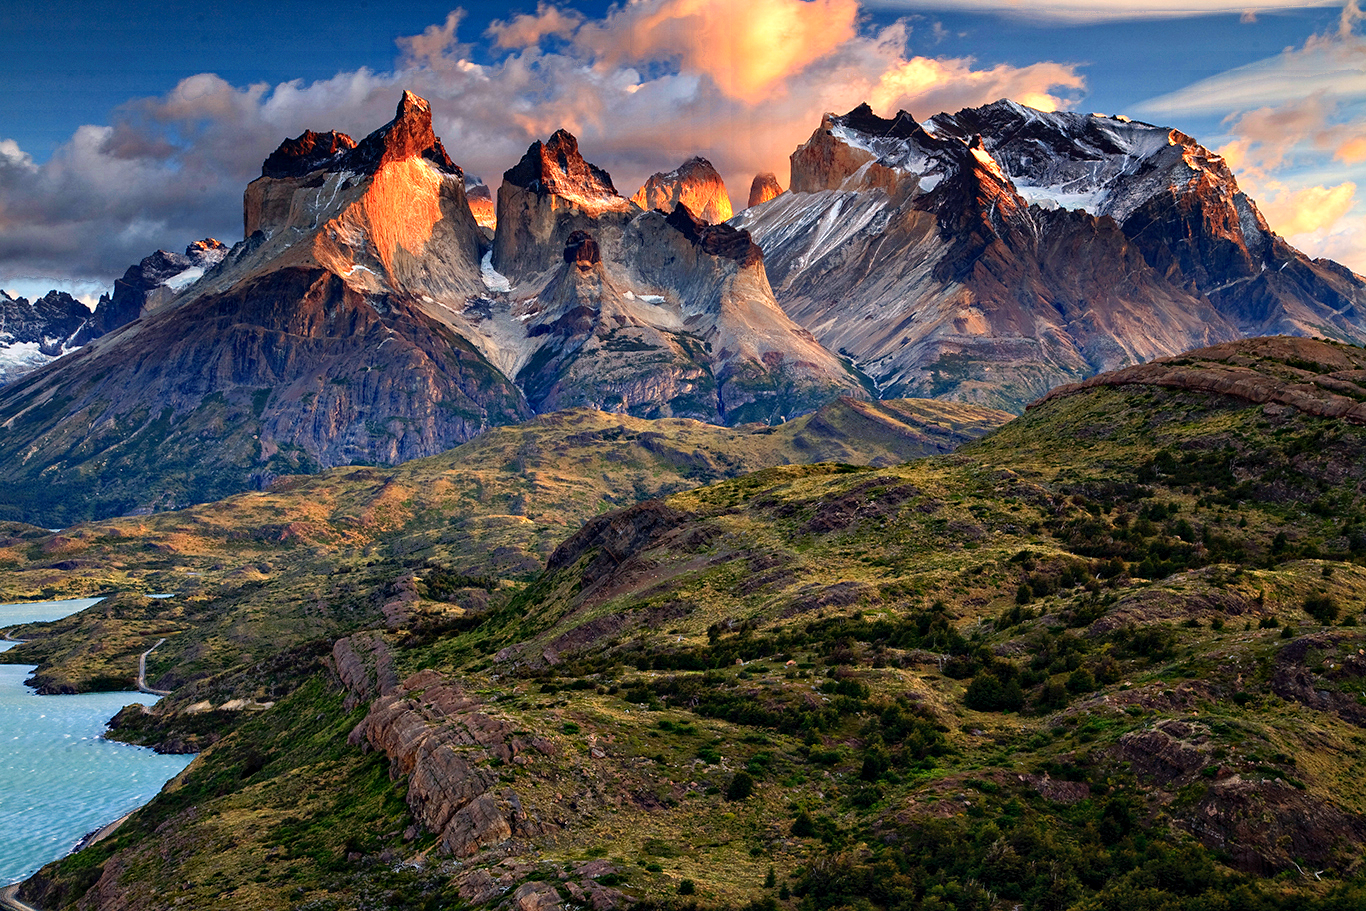
\includegraphics[width=0.45\linewidth]{..code/results/smoothing_landscape_sharp.png}
    \caption{Result of sharpening based on the smoothing.}
    {\it Left: original picture. Right: sharpened version.}
\end{figure}
}

{\small Photo of the Cordillera del Paine (Chile) by Gerad Coles, downloaded from the \textcolor{blue}{\href{https://www.gadventures.com/blog/12-of-our-planets-most-jaw-dropping-landscapes/}{website}} of GAdventures.}

\end{frame}

\subsection{Colorization}

\begin{frame}{Colorization}
    \begin{figure}
    \centering
    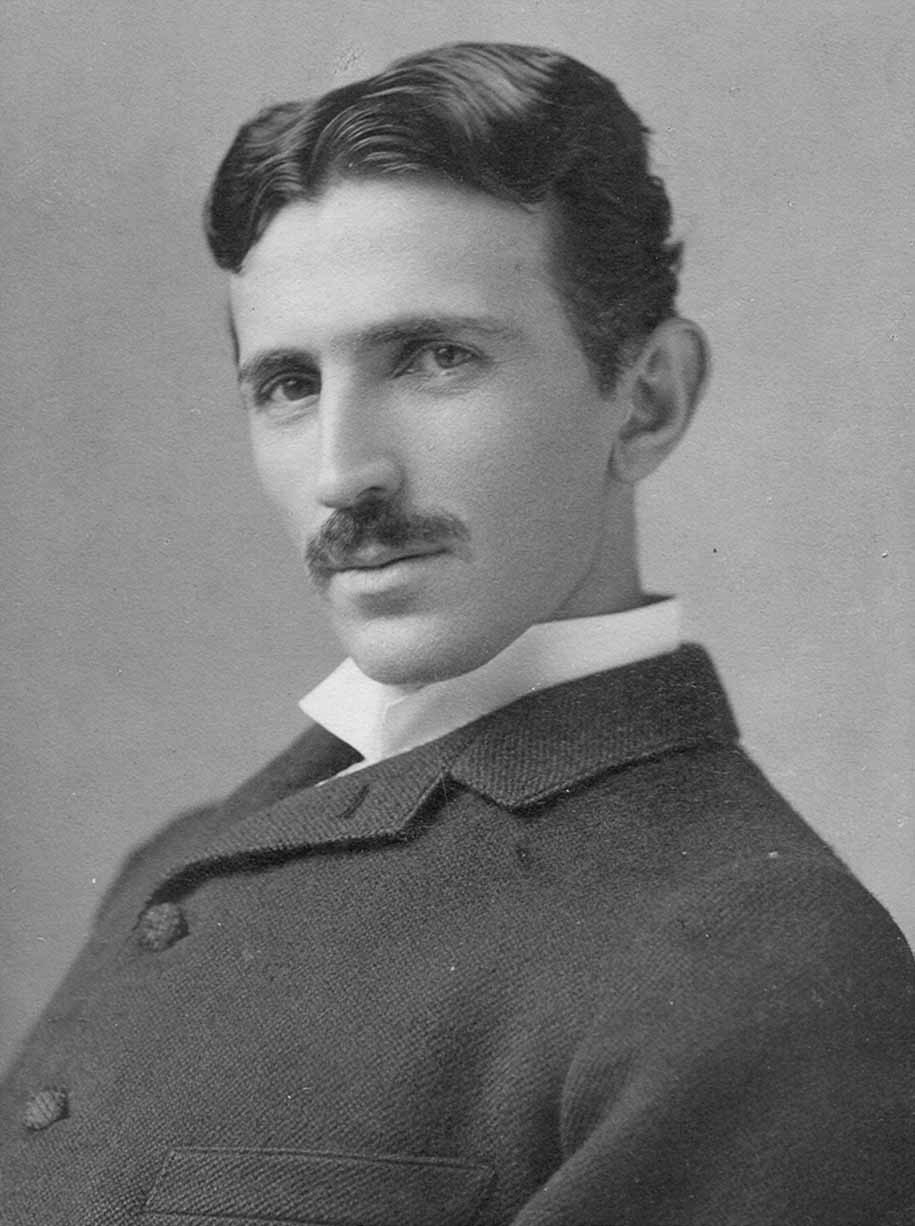
\includegraphics[width=0.3\linewidth]{..code/results/colorization_tesla_ref.png}
    \pause
    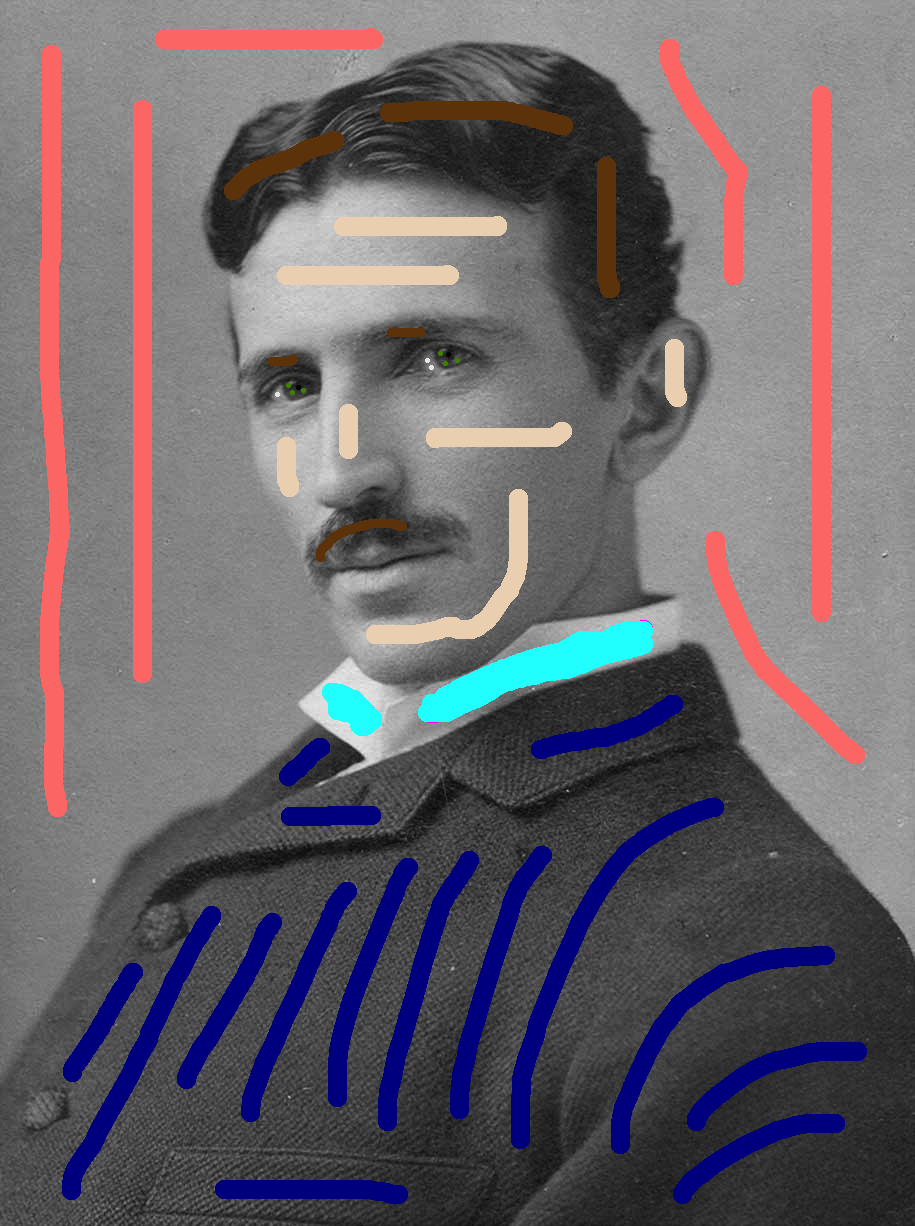
\includegraphics[width=0.3\linewidth]{..code/results/colorization_tesla_target.png}
    \pause
    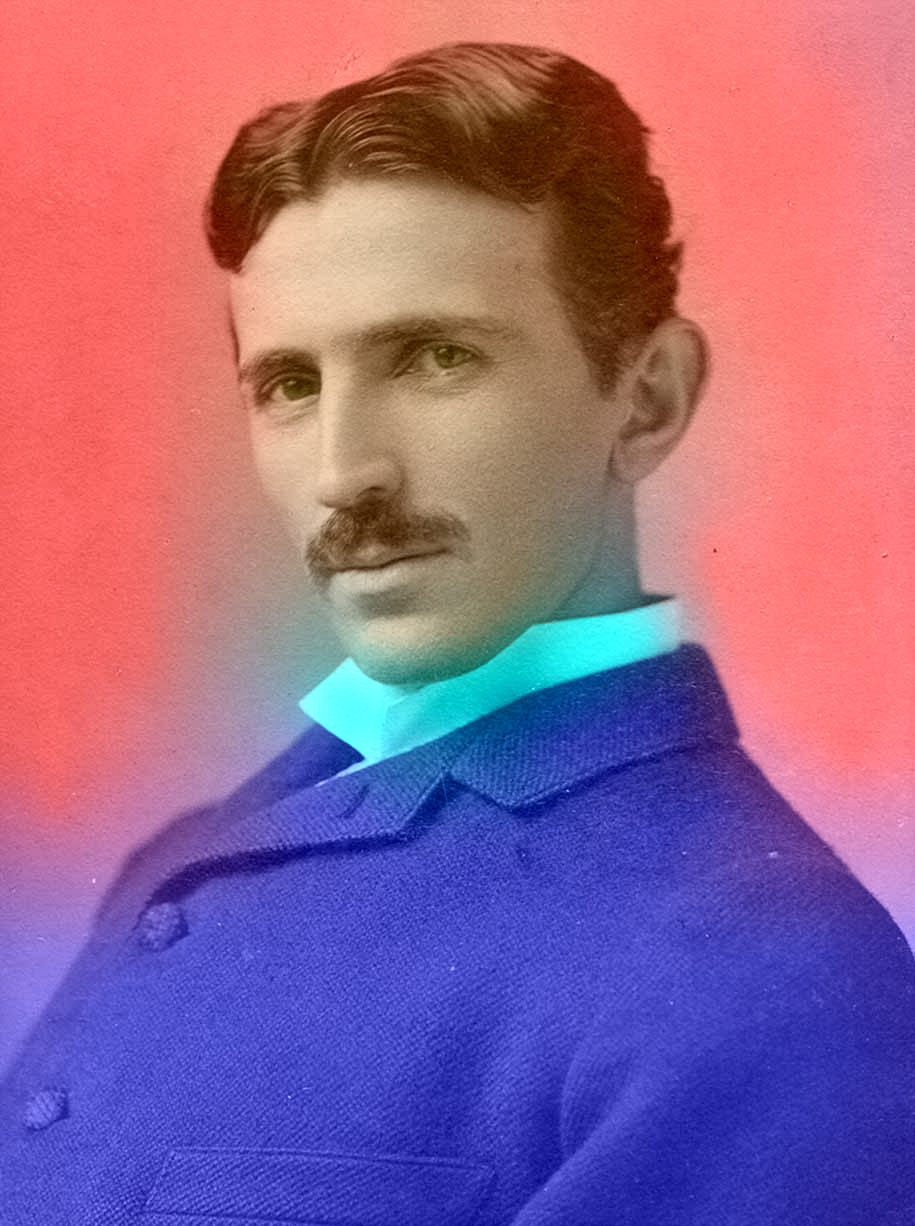
\includegraphics[width=0.3\linewidth]{..code/results/colorization_tesla_new.png}
    \caption{Result of colorization}
    {\it Left: original BW picture. Center: user markings. Right: result.}
\end{figure}

{\small Photo of Nikola Tesla by Napoleon Sarony (1893)}
\end{frame}

\subsection{Depth superresolution}

\end{document}